\section{Polynomial Spaces vs. Spline Spaces}\label{sec:p4}

\begin{enumerate}[(a)]
\item Figure \ref{fig:p4a} shows the graph of $s_0, s_1 \in U$
\begin{figure}[htbp]
	\centering
	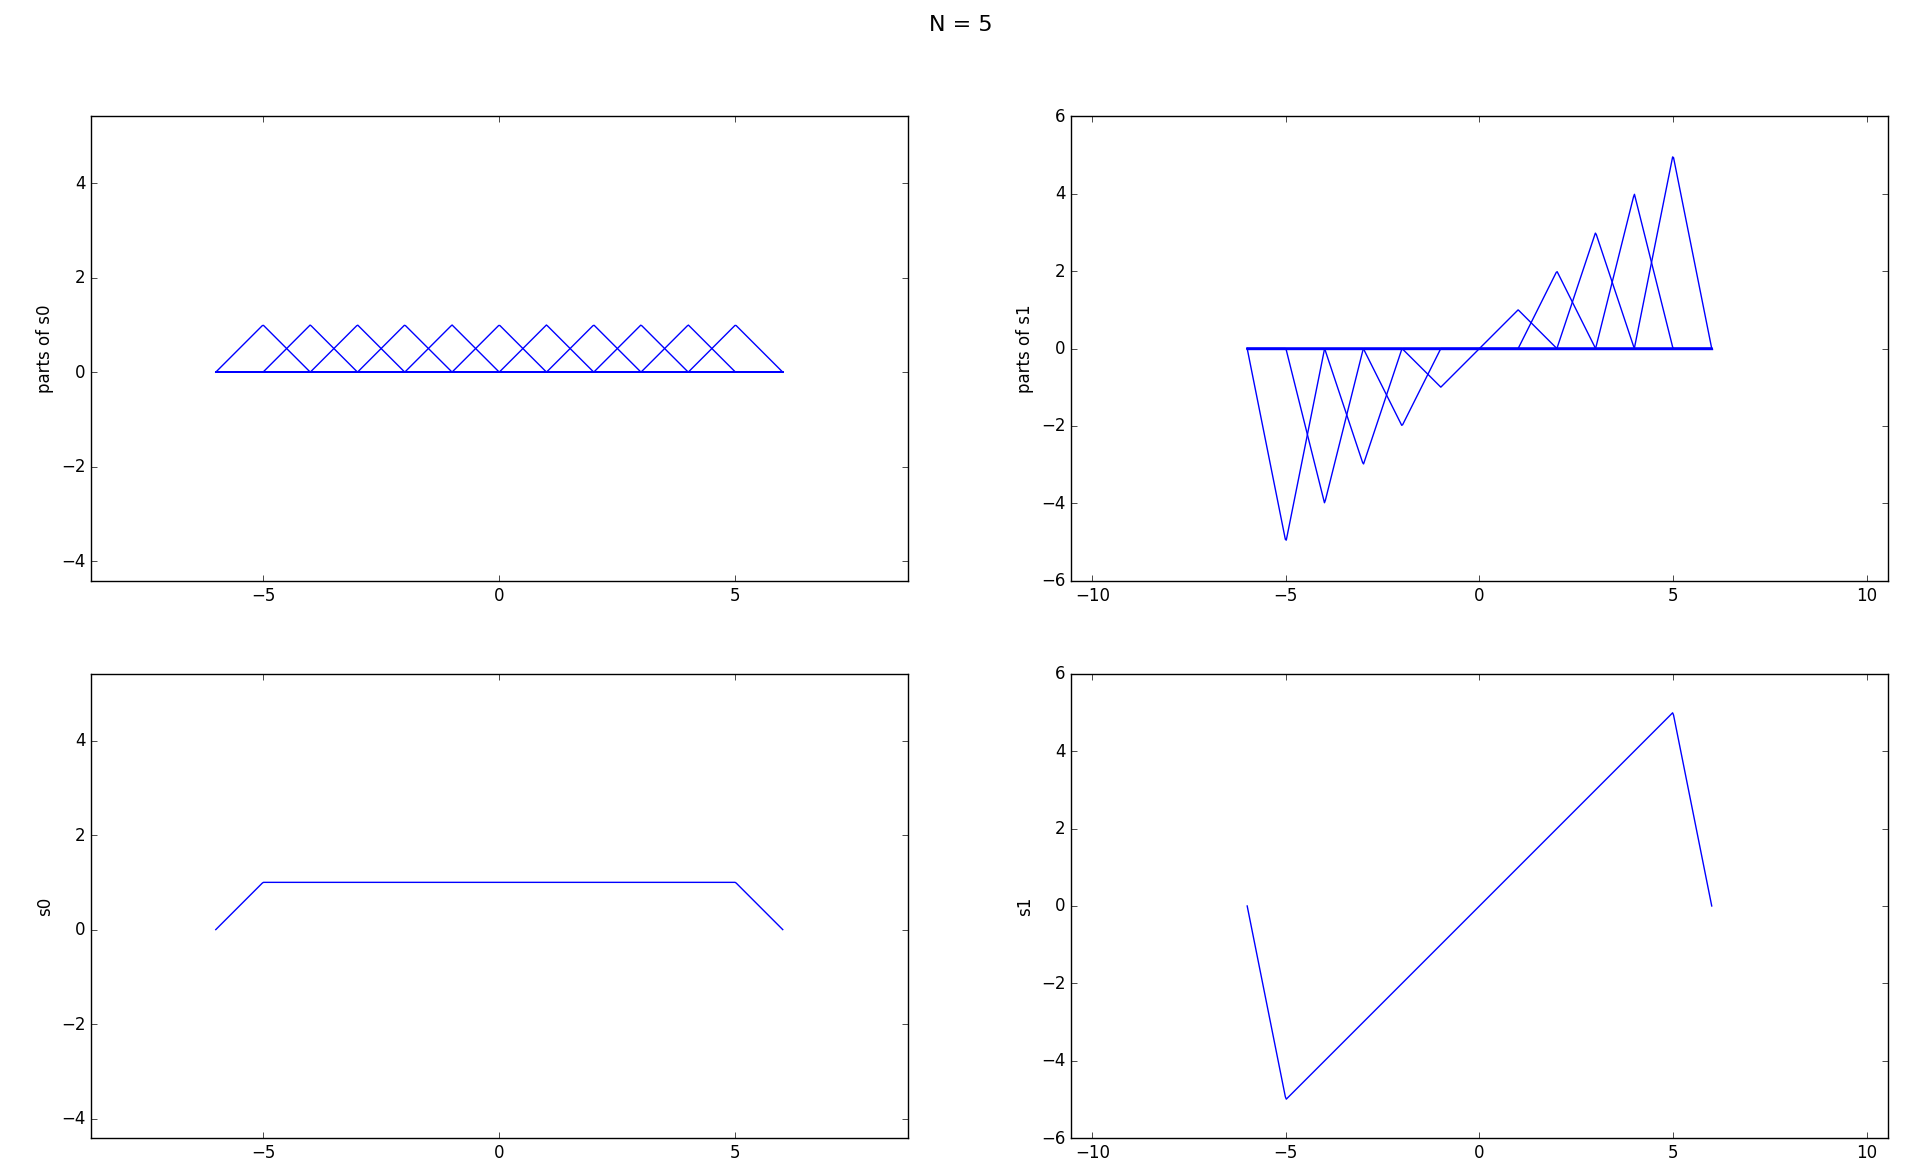
\includegraphics[width=\linewidth]{images/p4a}
	\caption{$s_0$ (left) and $s_1$ (right) with $N=5$}
	\label{fig:p4a}
\end{figure}

\item By inspecting Figure \ref{fig:p4a}, if we increase $N$, $s_0$ will approach $p_0(t) = 1$ and $s_1$ will approach $p_1(t) = t$. Hence, $p_0(t)$ and $p_1(t)$ are contained (as limit) in $U$.

\item $u_0, u_1$ belong to $U$  as well as $V_1$. However, $V_1 = \mathrm{span}\{v_0, v_1\} \Rightarrow \dim(V_1) = 2$ and $\dim(U) = \infty$. Hence $V_1 \neq U$.
\end{enumerate}